
\section{Preliminary Results}


\subsection{Case Study}
For our case study we want to analyse the problem of pick and place a movable object throughout a workspace containing a number of robotic arms. We represent the world using a cylinder (i.e beer can) as an object together with \textit{m} grippers connected to \textit{m} statically based robotic arms which allowed to move on a planner surface (i.e table). An example of a case consist of 5 arms is represented in figure \ref{fig:case_study}.

\begin{figure}[htb]
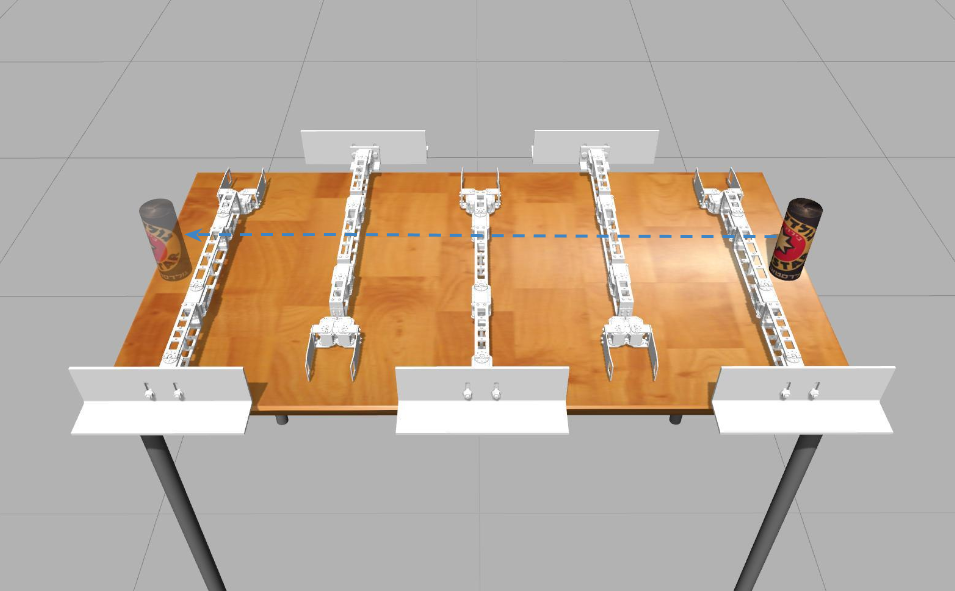
\includegraphics[scale=0.3,width=\textwidth]{5arms}
\centering
\caption{Case study Visualization} \label{fig:case_study}
\centering
\end{figure}


\subsection{Problem Formulation}
In this work our intention is to engage a single object pick and place problem using multi manipulators. We will handle the next symbols description for our problem statement. A manipulator will denoted as $A^{i}$ (the i'th parameter means the manipulator index) and an object as \textit{B}. We assume to have an overall of \textit{m} manipulators  $\mathcal{A}=\{A^{1},A^{2},\dots,A^i \dots,A^{m}\}$ and a single movable object. Furthermore we assume that each $A^i$ holds a workspace $W^{i}$ and a configuration space $C^{i}$ such that 
the Forward Kinematics (FK) is mapping $W^i$ from $C^i$ ($FK:C^i\rightarrow W^i$). Hence, the feasible workspace of the object will be then $\mathcal{W}^B=\{W^{1} \cap W^{2} \cap \dots  W^{i} \dots \cap W^{m} \}$ the overall \textit{configuration space} of the arms will be $\mathcal{C}^A=\{C^{1} \times C^{2} \times \dots  C^{i}  \dots \times C^{m} \}$  and the corresponding arm \textit{workspace} $\mathcal{W}^A=\{W^{1} \times W^{2} \times \dots  W^{i}  \dots \times W^{m} \}$ . 


For the purpose of consistency with \cite{koga1994multi,koga1992} we will presume the terminology of \textit{transit-path}, \textit{transfer-path} and \textit{manipulation-path} as follows:
\begin{itemize}
\item[\textit{transit-path}] is a path that describes a motion of an empty arm (i.e not grasping any object). We will use this term to represent a path of an arm which avoids collision with other arms or actually moving toward an object in order to grasp it.

\item[\textit{transfer-path}] is a path that describes a motion of an arm that is grasping an object within its gripper. We will use this term to represent a path of an arm that manipulates an object.

\item[\textit{manipulation-path}]  is a sequence of alternating \textit{transmit} and \textit{transfer} paths. We will use this term to represent a sequence of arms the moves an object from initial to goal positions.

\end{itemize}
Next, consider the following problem input:


\begin{itemize}
\item A set of $m$ robotic arms. 
\item Initial and goal positions of an object $B^{init},B^{goal} \in \mathcal{W}$
\end{itemize}
our objective is to find a \textit{manipulation-path} along which the object could be transferred according to input requirements. By definition each manipulation path is constructed by a sequence of \textit{Tspace} paths $\mathcal{T}^A=\langle T^{1},...,T^k, ...,T^n\rangle$ where $T^k \in \mathcal{W}^A$. In addition, each \textit{Tspace} path is derived by applying the FK rule on a sequence of $Cspace$ path. Therefore the corresponding \textit{Cspace} sequence of $\mathcal{T}^A$ resemble as $\mathcal{Q}^A=\langle Q^{1},...,Q^k, ...,Q^n\rangle$ where $Q^k \in \mathcal{C}^A$. This observation shows that any solution is obtained by calculating $\mathcal{Q}^A$ such that the equivalent $\mathcal{T}^A$ preforms a desired manipulation path. It is noteworthy that each $T^k$ is holding a $transit$ path for the entire arms (to operate in parallel) except one that holds a pair of $transit$ and $transfer$ paths for the actual manipulation.


\subsection{Planning Logic}

We let $\mathcal{T}^B$ be the object absolute path (i.e from initial to goal positions) such that $\mathcal{T}^B \in \mathcal{W}^B$, next we consider any $k$ element as a sub-task operation that moves the object along a portion of $\mathcal{T}^B$. Hence, we can reason that $\mathcal{T}^B$ is built up by a sequence of \textit{work-space} paths each handled on the $k$'th sub-task by a different arm, thus $\mathcal{T}^B = \langle T^B_1,...,T^B_k,...,T^B_n \rangle $. 

We define that object is restricted to move only when it is gripped, this aims the search 
to find a particular sequence of arms $S(k) \subset \mathcal{A} \mid [k=1..n] $ that will do the feasible manipulation job. Recall that any solution is represented by a sequence of $T^k$'s where each holds a path for the total arms. This means that $T^k$ is built by the set of $Tspace$ path of each individual arm $T^k = \{ T^{k,1},...,T^{k,i},...,T^{k,m} \}$. The resulted conclusion is an essential connection extracted between $\mathcal{T}^A$ and $\mathcal{T}^b$ such that for any $k$: $T^B_k = T^{k,S(k)}$.

We'll denote a $transfer~point$ as a position where any $T^B_k$ starts or ends (including $B^{init}$ and $B^{goal}$). Tentatively any $transfer~point$ located where an object is grasped or released by all of the arms in $S$. Any sequence $S$ consist of $n$ arms will have to pass through $n+1$ $transfer~points$ series $tp$. Assuring this condition is given by forcing any $T^{k,S(k)}$ to include $tp(k)$ and $tp(k+1)$ along their path. A summary of the general conditions for a valid $\mathcal{T}^A$ is as follows:
\begin{equation}
\label{eq:kinematic-feasible}
        \forall T^{k}: \{\exists Q^{k} \mid (T^{k} = FK(Q^{k})\} 
\end{equation}

\begin{equation}
\label{eq:consistant-sequence}
        \forall T^{k,S(k)}: \{ tp(k),tp(k+1) \in T^{k,S(k)}  \}
\end{equation}

\begin{equation}
\label{eq:no-collision}
        \forall T^{k}: \{ T^{k,i} \cap T^{k,j} = \emptyset \mid i,j=1..n~;~i\neq j \}
\end{equation}
where equation \ref{eq:kinematic-feasible} referring to kinematic feasible path, equation \ref{eq:consistant-sequence} is responsible for applicable sequence in terms of pick and place positions and equation \ref{eq:no-collision} imposing for having no collisions.





\subsection{Planning Process}
Recalling the work of Koga and Latombe \cite{koga1994multi}, it is shown that the object's world trajectory is the governing law when it comes to determine which is the grasping arm at any time. On the contrary we wish to give another perspective for the problem. Our guiding rule comes from shared workspaces of the arms. We are using the fact that any $transfer~point$ is located only in one of the shared workspaces and consequently $\mathcal{T}^B$ must pass through them. 

\begin{figure}[t]
    \centering
    \begin{subfigure}[b]{0.4\textwidth}
        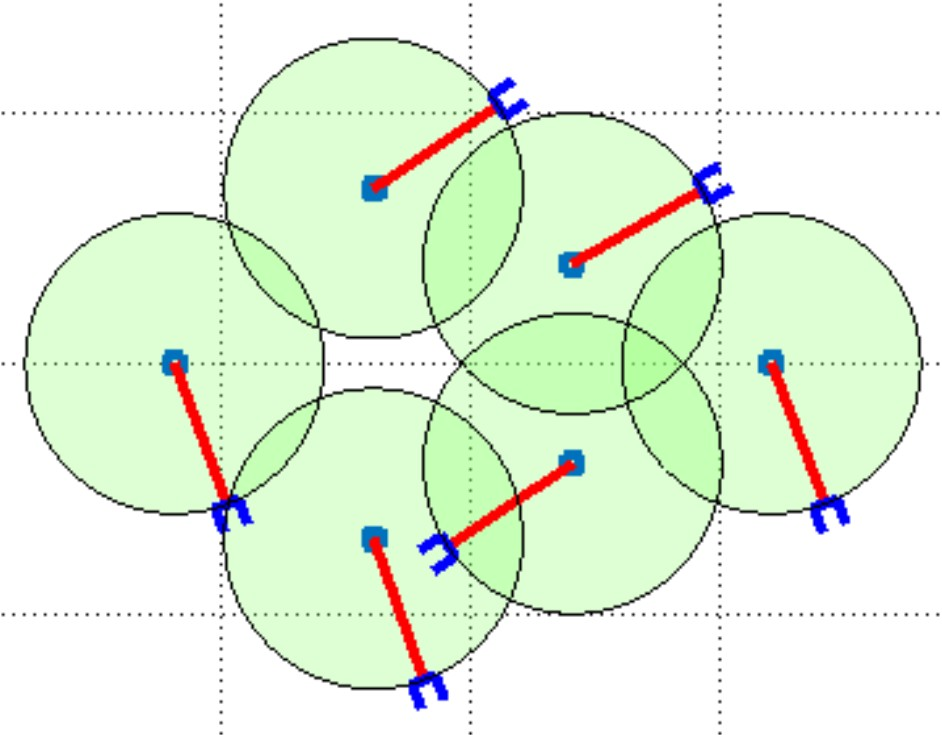
\includegraphics[width=\textwidth]{general_configuration}
        \caption{general configuration}
        \label{fig:general_configuration}
    \end{subfigure}
    ~~~~
    \begin{subfigure}[b]{0.4\textwidth}
        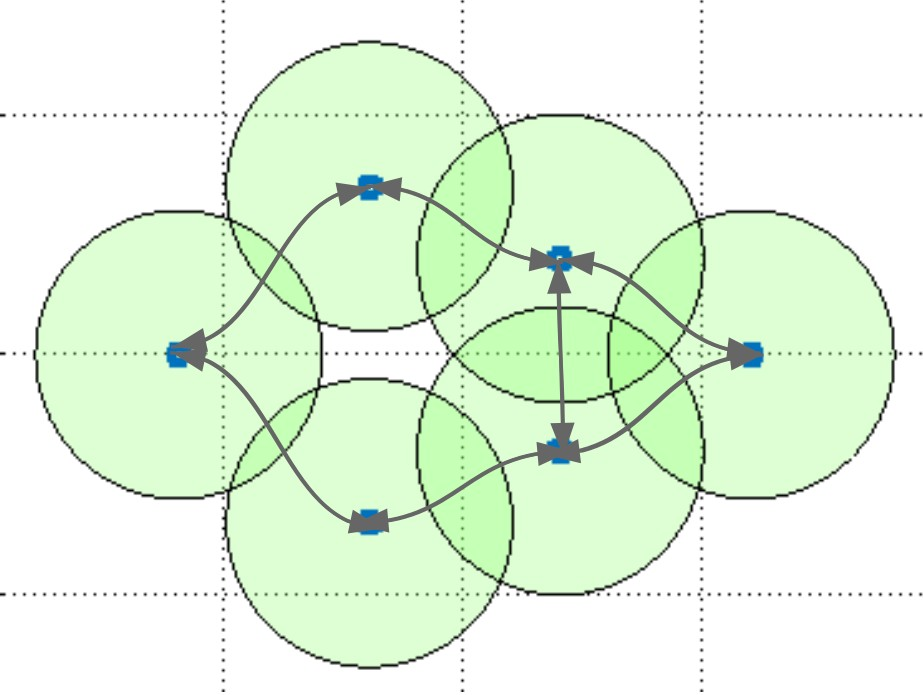
\includegraphics[width=\textwidth]{generated_graph}
        \caption{phase 1: generated graph}
        \label{fig:generated_graph}
    \end{subfigure}  
    
    \begin{subfigure}[b]{0.4\textwidth}
        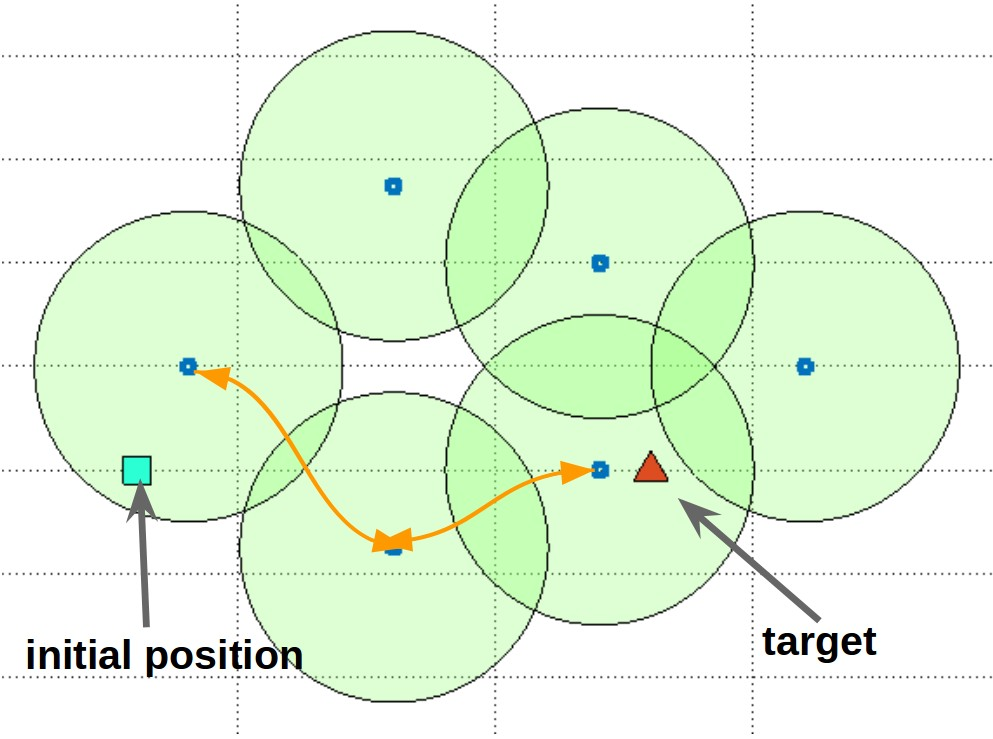
\includegraphics[width=\textwidth]{task_assignment}
        \caption{phase 2: Graph shortest path based on task properties }
        \label{fig:task_assignment}
    \end{subfigure}
    ~~~~
    \begin{subfigure}[b]{0.4\textwidth}
        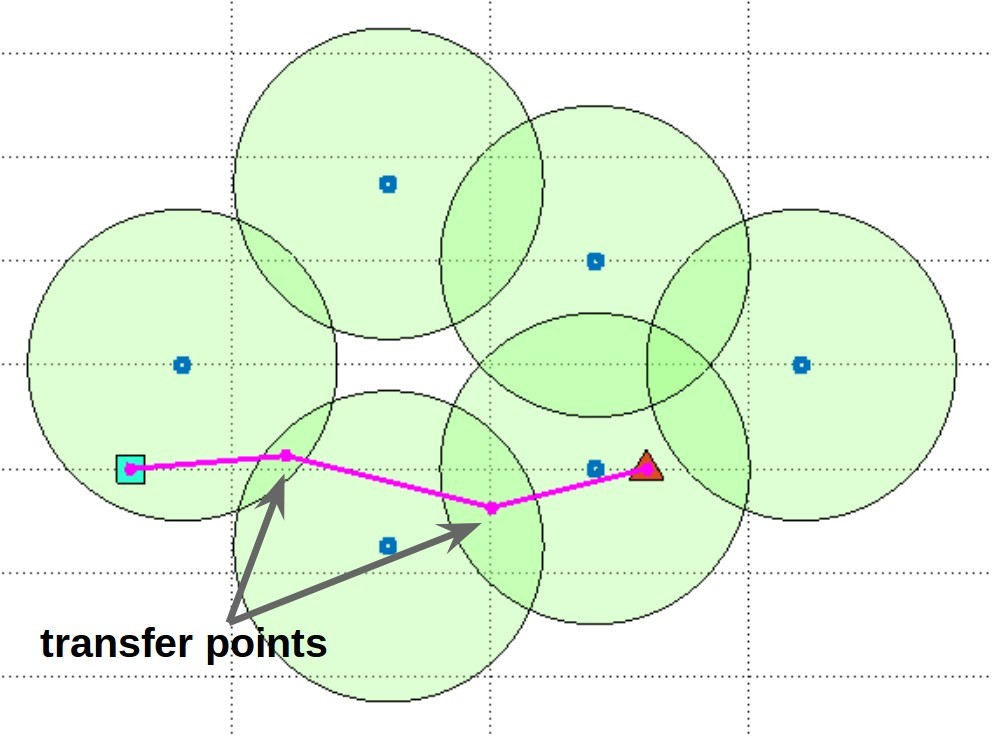
\includegraphics[width=\textwidth]{transfer_points}
        \caption{phase 3: calculating transfer points}
        \label{fig:transfer_points}
    \end{subfigure}
    \caption{Generating a sequence of arms and transfer points}\label{fig:animals}
\end{figure}

\subsubsection*{Search for Arm Sequence and Transfer Points}

One of the key component of our work is find any pair of arms sharing together a part of their workspace such that $W^i \cap W^j \neq \emptyset$, this fact gives an insight for any transfer that could appear. The easiest way to represent this data is by a graph where a node represent an arm workspace and an arc represents a shared workspace (between two arms/nodes). It means that a world consist of $n$ arms is interpreted by a graph with $n$ nodes where arcs are added on a second phase by checking any possible combination of shared workspaces. The generation of this graph will tentatively be called the $connectivity~graph$.

By attributing the initial and goal position of the object to one of the arms $Tspace$ we can reason about the starting and final node in the $connectivity$ $graph$. 
At this point, any graph search would give a solution with a form of a sequence of arms $S = \langle A^{first},...,A^k,...,A^{last} \rangle$ connected by their shared workspaces such that:
\begin{equation}
B^{init} \in W(A^{first})\mid A^{first}\equiv S(1)
\end{equation}
\begin{equation}
B^{goal} \in W(A^{last})\mid A^{last}\equiv S(n)
\end{equation}
\begin{equation}
W(A^{k})\cap W(A^{k+1})\neq \emptyset \mid A^{k}\equiv S(k)
\end{equation}
After generating \textit{S} the next task is to determine the position of a single \textit{transfer point} located in each shared WS. To do so a linear programming method will be used to minimize the total length accepted by connecting any pair of following \textit{transfer point} with a straight line.


\subsubsection*{The Search Algorithm}
To generate an actual sequence that will apply the condition as in equations \eqref{eq:kinematic-feasible}-\eqref{eq:no-collision} we will have to go through the steps as written in algorithm \ref{alg:main-loop}. The rationale behind this algorithm is first to find a sequence of arms $S$ together with a series of $transfer~points$ $tp$ that will settle with equation \eqref{eq:consistant-sequence} (lines 1-5). Next, when $S$ and $tp$ was determined the guidelines for a motion plan was resolved, thus the second phase of the algorithm was launched (line 6) in order to calculate the sequence path that meet equations \eqref{eq:kinematic-feasible} and \eqref{eq:no-collision}. 

\begin{algorithm}
\caption{Main Loop} \label{alg:main-loop}
\begin{algorithmic}  [1] % the [1] is for numbering
\REQUIRE $B^{init},B^{goal},\mathcal{A},q^{init}$
\ENSURE $traj$
	\STATE $cg\leftarrow GenerateConnectivityGraph(ws)$
	\STATE $W^{first}\leftarrow $ find($W^{first}$ such that $B^{init}\in W^{first}$)
	\STATE $W^{last}\leftarrow $ find($W^{last}$ such that $B^{goal}\in W^{last}$)
	\STATE $S\leftarrow$ BFS$( cg,W^{first},W^{last})$ // generate ws sequence
	\STATE $tp\leftarrow CalcTransferPoints( S,B^{init},B^{goal} )$
\STATE $\mathcal{T}^A \leftarrow CalcSequenceTrajectory( S,tp,q^{init})$
\end{algorithmic}
\end{algorithm}








\subsubsection*{Calculating Sub-Task Path}
As stated, at this stage our goal is to calculate the arms path for each phase of the \textit{manipulation-path} represented by $\mathcal{T}^A$. We assume that each phase includes the following input parameters (and that the initial configuration of the total arms is known):

\begin{itemize}
	\item Index of the moving arm.
	\item Initial and goal positions of the arms gripper
\end{itemize}

These parameters directs us to find a motion planning solution for a multi robot system. As mentioned in section \ref{section:motion_planning} there is no formal strategy for calculating optimal nor complete trajectory for multi robots except for using \textit{centralized} methods that suffers from exponential complexity. The pattern that we will next describe is a method that is designed to find a solution oriented for robotic arms but may still be used for other systems. 

The fact that a \textit{centralized} method includes complete and optimal attributes is that it can handle local minima's (same as A*). Lack in such feature resolved in having no reasoning when: robot 2 obstructs the path of robot 1 where actually robot 1 obstructs the path of robot 2 that should clear the path for robot 1. A simple illustration is shown in figure \ref{fig:initial_configuration} with a case of 2 robotic arms having 1 DoF each. The task here is to move arm \#1 to the dashed line. Trying to do so with applying any motion plan on arm \#1 only will result with "no solution" answer. It is obvious that arm \#2 needs to clear the way and the only option is to move counter-clockwise (moving clockwise is impassible due to the obstacle). 



\begin{figure}[t]
    \centering
    \begin{subfigure}[b]{0.3\textwidth}
    		\centering
        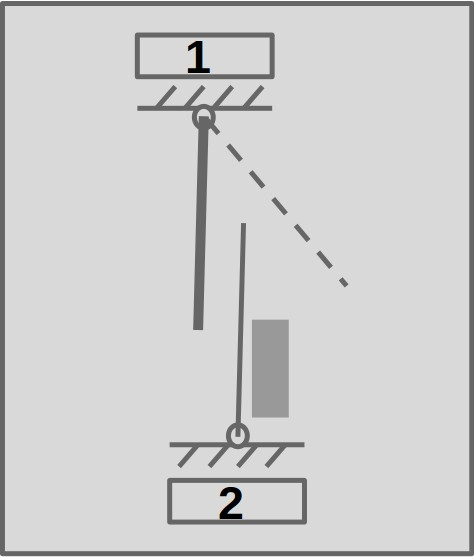
\includegraphics[width=0.8\textwidth]{initial_configuration}
        \caption{Initial configuration of the arms, goal of arm \#1 is dashed \\ }
        \label{fig:initial_configuration}
    \end{subfigure}
    ~
    \begin{subfigure}[b]{0.3\textwidth}
    		\centering
        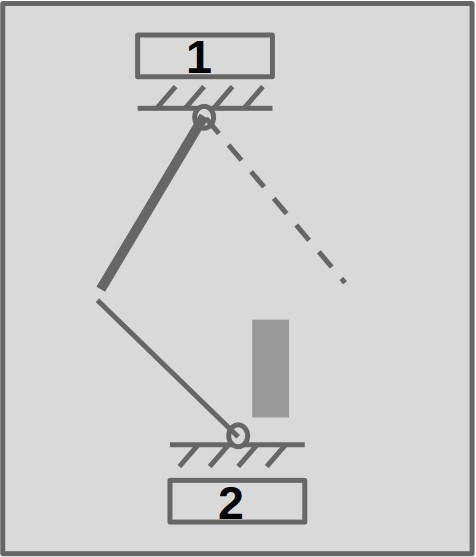
\includegraphics[width=0.8\textwidth]{breaking_point}
        \caption{A configuration of a "breaking point" from which the goal is reachable for a single arm task}
        \label{fig:breaking_point}
    \end{subfigure}  
    ~
    \begin{subfigure}[b]{0.3\textwidth}
    		\centering
        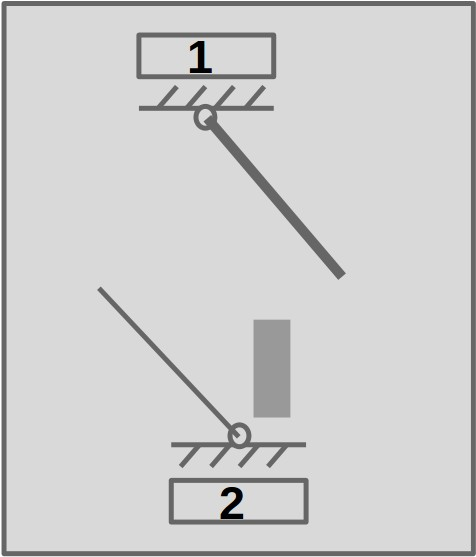
\includegraphics[width=0.8\textwidth]{final_configuration}
        \caption{Final configuration: goal achieved \\ \\}
        \label{fig:final_configuration}
    \end{subfigure}

    \caption{A multi arm problem configuration consist of 2 arms with 1 DoF each together with an obstacle (grey rectangle) that limits arm \#2 motion. In order to acheive the goal (figure c) a breaking point (figure b) must be acheived first. }\label{fig:local_minima_example}
\end{figure}


